% \documentclass[a4paper,twocolumn]{article}
\documentclass[twocolumn]{article}
\author{Andrew Haines}
\title{Wine Analyte Prediction using Neural Networks}
\usepackage[colorlinks=true, urlcolor=blue, citecolor=blue]{hyperref}
\usepackage{graphicx}	
\begin{document}
% generates the title
\maketitle
\section{Abstract}

It has been determined that certain analytes present in common wines cause negative variations in the perceived
quality of the products. The main compounds that adversely affect wine quality are 4-ethylguaiacol (4EG) and
4-ethyphenol (4EP). Enoses have become a cost efficient mechanism of monitoring for these analytes at the production
stage\cite{wineSpoilage}. In this project, 38 time series readings of a particular eNose (MOS-Enose) sensor in the presence 
of 38 different wines are provided with corresponding 4EG and 4EP values. The task of the project is to learn
a model that can predict 4EG/4EP values from MOS-Enose readings in the presence of an unseen wine. 8 such wine
measurements are provided and the purpose of the project is to provide predictions as to their analyte values.
This report details the approach used to provide such predictions.

\section{Initial Analysis of Datasets}

The first step in this project was to get a feel of the data to best plan an approach for how to
build the relevant prediction model\footnote{The source for the analysis is provided in the R file calibration\_analysis.r}
Looking statically at the provided readings, it is clear that the dimensionality of the dataset is huge. For each of the 12 sensors there 
is a reading twice every second for 600 seconds. Consequently, using the raw data as is, results in a model that has to consider $1200 \times 12$ 
dimensions. Such massive dimensionality would make a model incredibly susceptible to noise and 
overfitting especially in the presence of a small training set like the 38 training instances in this dataset. 
\begin{figure}[h!]
	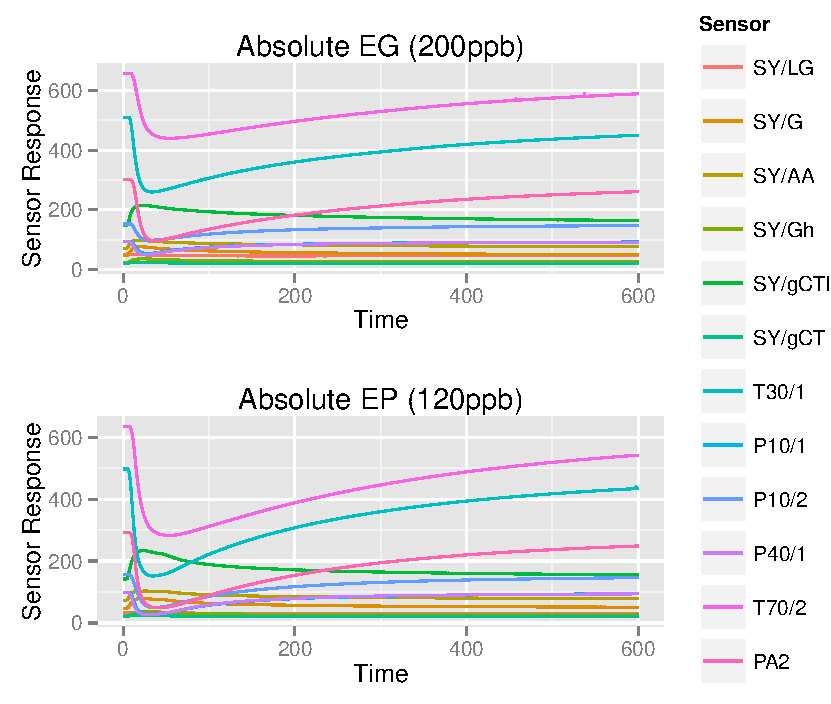
\includegraphics[trim = 0mm 0mm 0mm 0mm, clip, scale=0.55]{absoluteEGEPreadings.pdf}
	\caption{Absolute EG and EP readings of all sensors}
	\label{fig:absoluteAnalyteReadings}
\end{figure}
By performing pre-analysis on the dataset, insights into whether certain sensors are
redundant or correlated can be determined. If either of these properties can be found to be true then it is good evidence to suggest some
dimensionality reduction that can be performed on all data prior to being fed into the predictive model. \\
Provided as part of the dataset is a calibration set. Here, readings from various artificially constructed wine 
concentrations of 4EG and 4EP are measured to observe the effects on the sensors. Along with these readings, benchmarks 
are also provided of wine without any contaminants present. 
\subsection{Graphical analysis}
The first step taken was to simply get a graphical feel of 
how each sensor responds, over time, to the presence of each analyte (see Figure~\ref{fig:absoluteAnalyteReadings}
\footnote{Note that all data presented in this report is from averaged data of multiple readings of identical
experiments where available})

\begin{figure}[h!]
	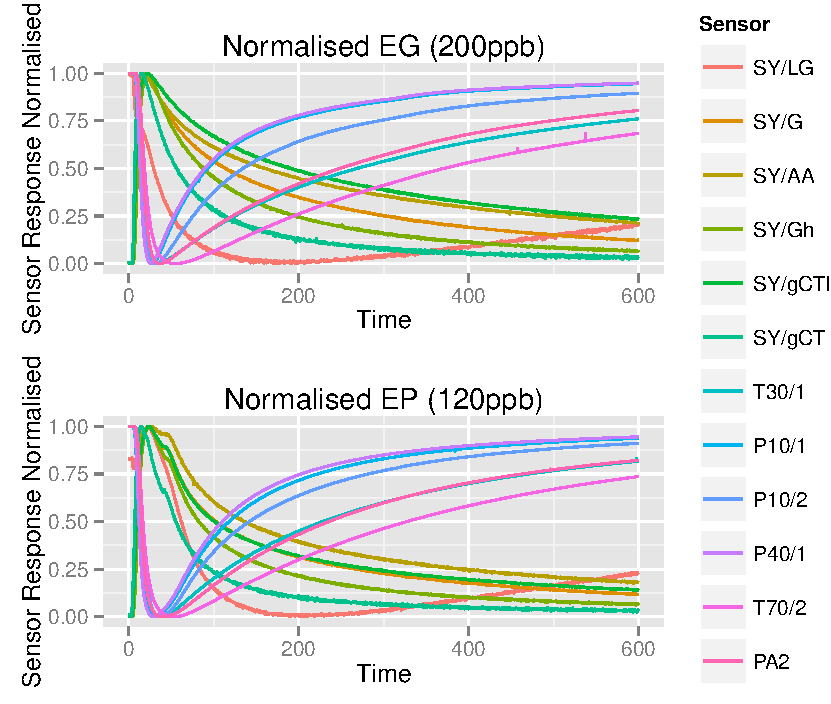
\includegraphics[trim = 0mm 0mm 0mm 0mm, clip, scale=0.55]{normalisedEGEPreadings.pdf}
	\caption{Normalised EG and EP readings of all sensors}
	\label{fig:normalisedAnalyteReadings}
\end{figure}
Here it can be seen that the sensors clearly take time to react with the wine (probably due to
diffusion of the aroma particles from the wine to the sensors). Moreover, at first glance it appears that
certain sensors react more than others. This observation is based on the assumption that the scale that
each sensor operates on is the same. If these sensors do not operate at the same scale then such a statement
could be a very dangerous falsehood. Considering the normalised representations of these readings we can
see that certain detectors contain a higher area under the graph which may be representative of that sensor
reacting more then others. This shall be explored later. Also observable in these charts is that the data is quite noisy. 
To combat this, kernal smoothing (using Nadaraya–Watson kernel regression estimates\cite{nwkernal}) has been applied to all further 
datasets in this report to smooth the noise out.\\
The next step is to consider how the sensors behave as a difference from the baseline. The idea here is to try
and isolate the sensor reactions that respond to the analytes themselves. Background odours from the wine and its
environment are going to be contributing factors to the sensor measurements. By removing the baseline readings (where no analytes
were present) an approximation can be derived for the relative target compound reactions. This requires a look
at the relative readings when the baseline has been subtracted (see Figure~\ref{fig:absoluteAnalyteDiffReadings})
\begin{figure}[h!]
	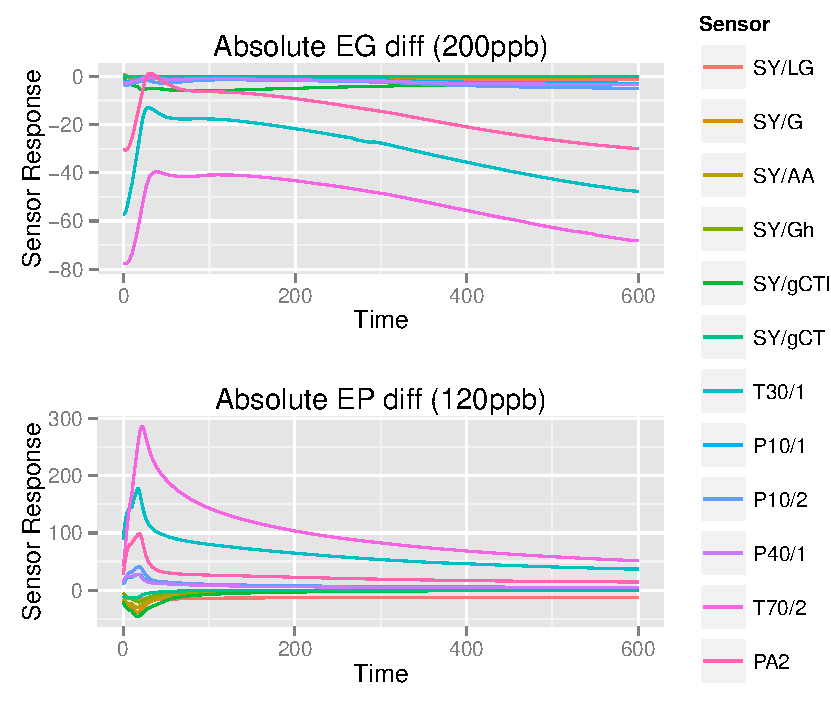
\includegraphics[trim = 0mm 0mm 0mm 0mm, clip, scale=0.55]{absoluteEGEPDiffreadings.pdf}
	\caption{Absolute EG and EP readings of all sensors with baseline removed}
	\label{fig:absoluteAnalyteDiffReadings}
\end{figure}
\begin{figure}[h!]
	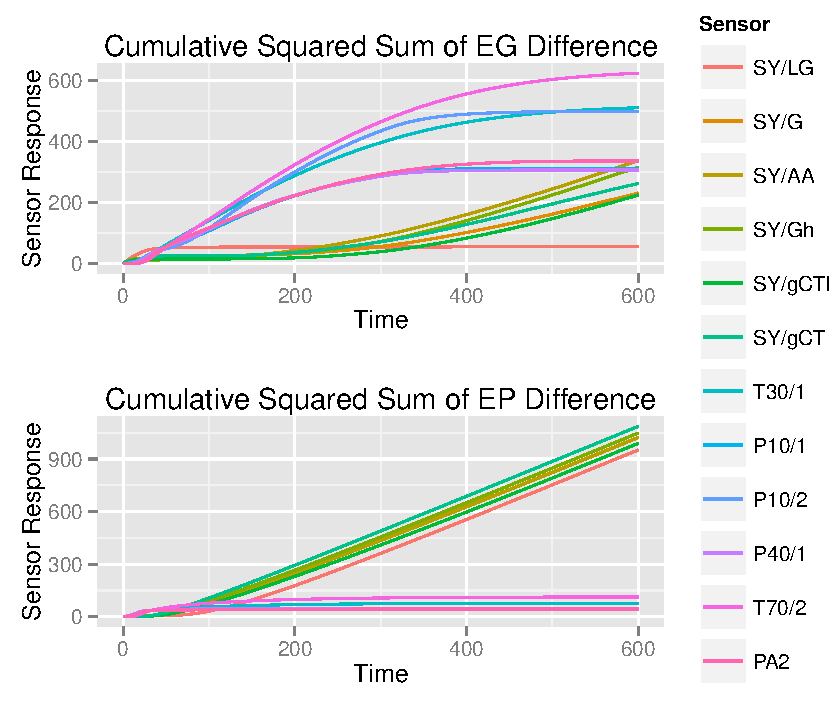
\includegraphics[trim = 0mm 0mm 0mm 0mm, clip, scale=0.55]{cumulativeSquaredSum.pdf}
	\caption{Monatomic Cumulative Squared plot of normalised EG and EP readings of all sensors}
	\label{fig:cumulativeSquaredSum}
\end{figure}

Observing the effect of the difference over the relative baselines gives an indication that certain sensors
are simply not reacting to the target compounds. From this analysis it appears that sensors PA2, T30/1 and T70/2
are stimulated the most. What is also apparent from this representation is that there is an indication that
these sensors are correlated (co-insides with the conclusions of \cite{wineSpoilage} and \cite{MOSAnalysis}). As one increases, so do the others. It can also be seen here how the sensors differ in
the presence of 4EG and 4EP. 4EP appears to cause the sensors to increase their relative measurements whereas 4EG
dampens the sensor's responses. This implies that the presence of the 2 substances could be at odds with each other.\\
Also, although these mentioned sensors do appear to react heavily to the presence of the target analytes, it again is 
on the assumption that the operating scales of the sensors are consistant. As none of the other sensors are absolutely zero 
(except for maybe SY/gCTI) at this stage it is still not possible to conclude that they are not contributing information that could be used in the prediction model. As mentioned
previously, looking at the integral of the normalised datasets might be useful to gauge how much 'power' each sensor has over the others
when all normalised between 0-1. To visual demonstrate this analysis a cumulative squared summations\footnote{squared to remove negative values offseting 
the monotomic requirement of this analysis} of the baseline removed datasets were considered (see Figure~\ref{fig:cumulativeSquaredSum}. 
The results show that there are indeed some sensors that dominate over others for the presence of the various analytes. Sensors such as SY/LG 
clearly provide little information whereas T70/2 dominates for EG reading. At first glance it feels that a threshold could be set and all
sensors that exhibit a total reading below that should be excluded but this doesnt help remove the correlations that are clearly visible
in this dataset. It is clear that graphical analysis of the data is not enough to conclude if any sensors are redundant and more analytical 
approaches are required.
\subsection{PCA}
Principle Component Analysis is a process of projecting a dataset into a new space, represented as projections
from new orthogonal basis vectors (eigenvectors)that separate the data dimensions so no correlations are present in the new
space. Such a technique can be used to rotate a dataset onto this new completely 
othogonal space with zero mean and unit variance (whitening transform\cite{whitening}). Doing so means that each dimension
is in the same scale (normalised) and expresses the maximum amount of information for that dimension\footnote{correlated dimensions
in a sense share information and therefore are not as expressive as 2 dimensions that are uncorrelated}
Furthermore, by looking at how the projections (or scores) of the original dataset on these new basis vectors vary (the variance), it can be
easily observed which of the new dimensions contribute the most information of the dataset. Dimensions where the projections
vary alot(high variance) imply that there is alot of information in this dimension. Dimensions where the projections do not
vary much means that this dimension tells little information about how the data set evolves. Using this, components that
hold little information can be removed from the data and thus the total dimensionality of the dataset can be reduced. 

\begin{figure}[h!]
	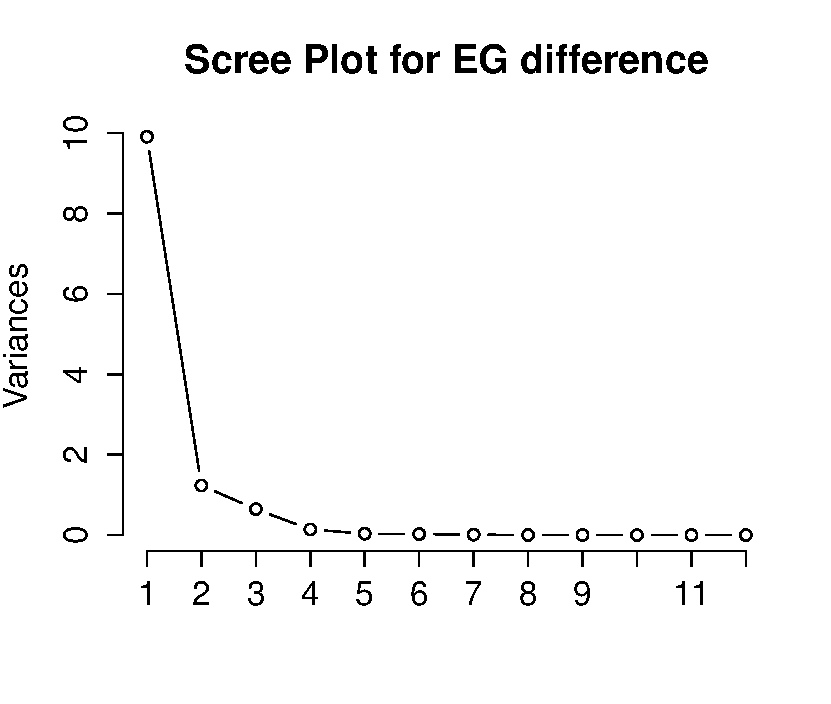
\includegraphics[trim = 0mm 0mm 0mm 0mm, clip, scale=0.6]{EGScreePlot.pdf}
	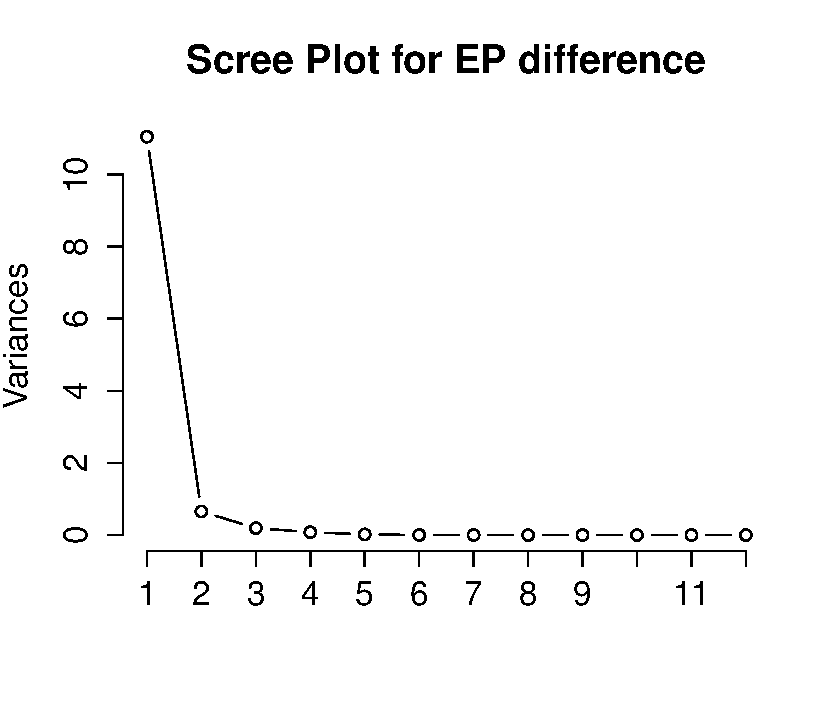
\includegraphics[trim = 0mm 0mm 0mm 0mm, clip, scale=0.6]{EPScreePlot.pdf}
	\caption{Scree Plot for EG/EP readings showing PC variances}
	\label{fig:screeplot}
\end{figure}
From studying the results of the PCA analysis on the EG difference results, it can be seen that PC1 contains $0.8258$ of the total variance, 
whereas PC2 contains $0.1027$. The rest of the components account for an accumulated $0.0715$ suggesting that these can all be discarded as 
they dont contain much useful information. Using the kaiser criteria also confirms that only PC1 and PC2 need to be kept as they are
the only components that have eigen values above 1. \\
Looking at the EP difference data tells a similar story but this time PC1 contains the majority of the information of the dataset with
a $0.9209$ proportion of the variance. Again the scree plot and kaiser criteria suggest that PC1 need only be kept(see Figure~\ref{fig:screeplot}). 
As another visual aid, the biplots show in Figure~\ref{fig:biplot} show how the time samples vary around the components\footnote{To make the results
more visible, the datasets have been desampled to 1 sample every 4 seconds, with values averaged between samples. See Section ~\ref{sec:desampling}}. Also on the plot
are the relative sensor loadings that point in the direction of the PC they attribute to the most. With the EP plot, we can see that the sensors
appear to be separated into two opposing directions on the PC1 axis. This fits with the findings that PC1 carries the majority of the information.
With the EG plot on the other hand the same effect can be observed except for the SY/LG sensor that points directly in the PC2 direction. Thus it can
be concluded that EP just requires PC1 whereas EP requires both its PC1 and PC2 components.\\
To summarize, by performing PCA on the data, the new feature space can represent the data in a consistant scale (removing the issues experienced 
using the graphical methods) and also provides the majority of the information in 3 principle dimensions (2 for EG and 1 for EP). Projecting a 
dataset onto these components greatly reduces the dimensionality of the dataset 
\begin{figure}[h!]
	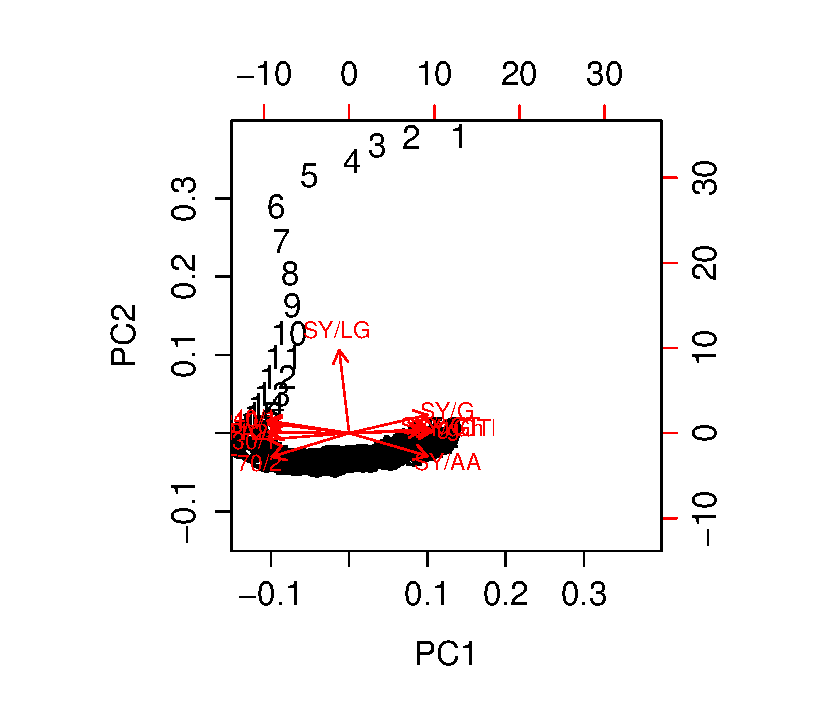
\includegraphics[trim = 0mm 0mm 0mm 0mm, clip, scale=0.55]{EGBiPlot.pdf}
	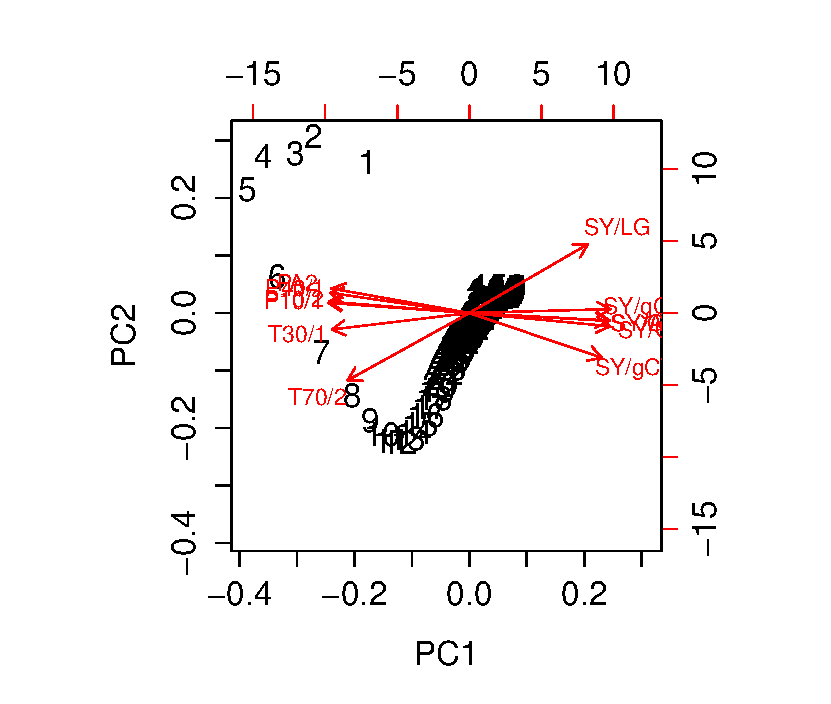
\includegraphics[trim = 0mm 0mm 0mm 0mm, clip, scale=0.55]{EPBiPlot.pdf}
	\caption{BiPlot for EG/EP Main Principle Components}
	\label{fig:biplot}
\end{figure}
\subsection{Desampling}
\label{sec:desampling}
As already mentioned, using PCA, the new feature space has reduced the dimensionality to just 3 principle components. Given that there are still
1200 readings for each of these dimensions, this still leaves a total feature set containing 3600 features. More work is needed
to reduce it further. Currently the data is sampled at 2Hz meaning there are two readings every second. By desampling to a lower 
frequency and averaging the replaced samples, the dimensionality can be greatly reduced. To determine the correct degree to what degree of desampling 
should be performed, PCA can be considered again.\\
The intuition here is that the dataset should be desampled as much as possible but only so much that the variance of the determined PCs
does not drop too much. Too much in this case is so that the kaiser criteria is still up held to the point that EG (PC1,PC2) and EP(PC1) are still
the dominent components (it might be possible to desample even further but then include more PC's but this will be left as possible future 
areas of study). Further to this, although values of $\textless 0.025Hz$ (one reading every 40 seconds - see Figure~\ref{fig:desampledExample}) 
seem to maintain similar variance values of the PCs being considered, The performance of the model will be evaluated with different desampling
values to tune this parameter appropriately. More on this is described later. As a guidance, resampling at 0.025Hz provides a $3 \times 16 = 48$ 
total dimensionality model. Something much more manageable then the original dataset.

\begin{figure}[h!]
	\includegraphics[trim = 0mm 0mm 0mm 0mm, clip, scale=0.55]{deSampledExample.pdf}
	\caption{Example of desampling the EG difference plot to 0.025HZ. The main structure of the data is still present}
	\label{fig:desampledExample}
\end{figure}

\section{Learning a model}
Now that the data has been analysed and a proposed workable dataset with $\approx48$ dimensions, an appropriate prediction model needs to be chosen.
Due to the computationally efficient learning and prediction phase, its intuitive geometric representation and simply because i have never
implemented one before, the RBF neural network has been chosen for this prediction problem. Before discussing implementation details
of the network itself, based on the findings from the previous section, a preprocessing layer is required for all data into the network
to transform its high dimensional space into something more manageable. 
\subsection{PreProcessing}
The next stage of this project was to perform a consistant series of steps to transform all data (both training and prediction sets) into a
feature space more concise and informative than the original dataset provided. The reduction transformation steps have already been discussed so the 
following serves as a formal reference to the pre processing steps used. It is worth pointing out however that the following steps are no longer 
performed on the calibration dataset (unless explicitly stated) but on the training and prediction sets as they enter the model. The order that the 
processing occurs is as presented. These steps can be found in preprocessing.r and preprocessing-utils.r R source files.

\begin{enumerate}
	\item All data is smoothed using Nadaraya–Watson kernel regression estimates
	\item All data is subtracted from the calibration set's baseline readings (average of both 4EG and 4EP readings)to reduce impact from 
		  other properties of the wine and its environment.
	\item All data is downsampled to $x$ Hz where $x \textless 2$. This value is a free parameter that will be evaluated as part of the network's performance.
	\item PCA basis vectors of desampled calibration dataset calculated 
	\item All data is projected onto the loadings from the PCA basis vectors \footnote{The loadings used are from both the EG and EP analysis. First the
		  data is rotated in the EG space. Next the original data is then projected into the EP space}.
	\item The latent components of the two projected dataset (one for EG one for EP) are then removed leaving only PC1 and PC2 for the EG projection
		  and PC1 of the EP projection.
	\item EG and EP projections are then merged together to create the complete pre processed input data
	
\end{enumerate}

\subsection{Network}
The network used in this project is an RBF network with $k$ k-means positioned prototypes and it's implementation is provided in the network.r R source file. 
The general principle of the network is that a training set is used to cluster $k$ centers or prototypes around the instances. Each prototype
has a position in the feature space that radiates a field around it. When an instance is to be classified it is positioned in the feature space according
to the values assigned to it. The position of this instance will sit in the radius fields of the prototypes defined with each field's strength being
proportional to the distance from the instance to the field's origin prototype. The strength of the field will determine how much that instance is
influenced by the prototype and it's influence is then multiplied by a learned weight attributed with the prototype. An instance can and most likely 
will be positioned over a number of fields so the overal output of the network is the summed value of all weighted prototype influences.\\
The centers are of the prototypes are positioned using the k-means algorithm whereby $k$ randomly generated clusters (in the bounds of the min/max 
values of the instance set used) are iteratively moved towards clusters in the dataset. These clusters are defined by assigning 
membership of instances to the prototypes using the L2 norm distance:
\[
\|x\| = \sqrt{\sum_{i=1}^{N}(x_i - y_i)^2}
\]
The prototype with the lowest distance to an instance (closest) is the prototype that gains this instance as membership. After each instance
is assigned to a prototype, the mean distance of all prototype members is computed and the prototype is moved to this position. Membership is
recomputed and the prototypes position moved until no more movement occurs. \\
An implementation consideration is what happens when a prototype does not have any members after the algorithm finished. A simple approach would
be to simply remove the empty prototypes but this could, due to the starting initial conditions being random, mean that all instances could be
assigned to a few prototypes, meaning that we have less positions to model our training data. As the dataset is very sparse (only 38 training
instances), having less then $k$ prototypes would have a large impact when measuring the performance of the network (especially when evaluating what
$k$ value to use itself). Consequently a recursive implementation that retries the algorithm until each prototype is assigned a member. Although this
scheme is a little brute force, in practice this doesn't add any noticeable overhead when $k\ll|instances|$\footnote{See conclusion section for more 
on this effect. After experimentation, this statement is not entirely true as the lack of instances means that from a probabilistic perspective,
it becomes more and more unlikely to not have an empty prototype as $k$ increases and thus this adds huge computational overhead}. A better scheme using an optimization
approach might be more appropriate if the instance numbers are much larger.\\
\\
Once the prototypes have been defined and positioned, a radial basis function needs to be applied to them. For this project, a gaussian implementation
of the form is used:

\[
 \phi(x) = \exp(-\frac{\|x\|^2}{2 \times \sigma^2})
\]

The sigma used is calculated in either two ways. If there are enough instance examples (currently set to \textgreater 50), then the covariance 
matrix of the actual instances are used\footnote{If there are not enough instances, the covariance matrix can heavily overfit the data provided to it
hence why there are two schemes in this implementation}. If there are \textless 50 (which will always be the case with this training set) then the sigma of the
gaussian is set at a constant width proportional to the maximum distance between any 2 prototypes in the network (to ensure every prototype can
'reach' any instance in the feature space). The sigma used is defined by 

\[
\sigma = d_{max} / \sqrt{2 * k}
\]

Its worth mentioning that because of the normalising whitening step used as part of the PCA preprocessing, the instances fed into the network will
have 0 mean and unit variance meaning that the gaussian function will not need to use any skewed covariance matrix hence it should be acceptable
to use the global sigma calculation.\\
Once the functions have been set up on the prototypes, the next step is to learn the weights of the network. This is accomplished arithmetically
by minimising the error terms (expected - actual) in the quadratic sense. Using an adaptive form of the psuedo inverse matrix transform (single
value decomposition) multiplied by the expected values ($\underline{D}$), the weights can be calculated with an error penalty $\lambda$ term to help 
aid smoothing the error rates and thus help increase generalisation. The complete learning stage is performed using Poggio \& Girosi's 
regularization applied form\cite{poggio}:

\[
\underline{W} = [\Phi^T \Phi + \lambda I]^{-1} \Phi^T \underline{D}
\]

\subsection{Determining Free Parameters}
As already noted, this network contains a number of free parameters that need to be fixed prior to training and predicting phases.
In summary, these parameters are:

\begin{enumerate}
	\item $n$ Hz desampling rate
	\item $k$ prototypes
	\item $\lambda$ error penalty term
\end{enumerate}

To evaluate the best possible combination of these values prior to predicting the unseen dataset, a N fold cross validation scheme is
used. This process involves taking the 38 training instances and randomly splitting them into n equal bins. The process works by iterating over the
bins, one by one, using each bin in turn as a test set and the rest of the bins as the training set. This continues until every bin has been
considered as a test set. The error rates of each iteration are then averaged using mean squared error of the actual vs predicted output of the network
and this value is deemed the overal error rate of that particular network (and its configuration). The idea here is that the performance of the 
network is evaluated on all combinations of instance training to test sets rather then just only potentially lucky/unlucky combinations. 
Due to the fact that the training set is so small, having as many instances in the training fold is most important. For this reason, 
18 fold X-validation was used. This equated to 18 tests of 36/2 train/test splits. The implementation is provided in evaluation.r and network.r.

\section{Performance results}
After letting the evaluation run to completion, it determined that that the best values for the free parameters are:

\begin{center}
	\begin{tabular}{| p{15mm} | p{15mm} | p{15mm} | p{15mm} | }
	\hline Parameter & $error_{min}^2$ & $error_{max}^2$ & $error_{avg}^2$\\ \hline
	\( k=25\) & 130 & 231300 & 32970 \\ \hline
	\( n=20 - 93D\) & 130 & 231300 & 32970 \\ \hline
	\( \lambda\) & 130 & 231300 & 32970 \footnote{These values were all determined from the same optimal iteration hence why they are all the same}\\ \hline
	\end{tabular} 
\end{center}

The choice of the parameters was driven by the $error_{avg}$ whereby the parameter that generated the lowest average error was deemed the
best\footnote{There are two evaluation scripts considered in this project. $evaluate1()$ evaluates all combinations of all parameters to ensure 
that every parameter is considered. The idea being that if the parameters are not independent then there is an optimal configuration of 
textit{all} parameters. Due to the exponential $O(k^{n^{\lambda}})$ nature of evaluate1 in evaluation.r, it simply took too long to execute. 
evaluate2 on the other hand evaluates each parameter one by one, holding the other parameters consistant. This implies that the parameters 
are independent but does complete in $O(k+n+\lambda)$}. Output of the evaluation scripts is presented in performance-results2.txt. It is worth
noting, that using higher dimensionality feature spaces takes a lot of time to train (\textgreater 20 mins).\footnote{See conclusions section
about posible issues with this process}

\section{Wine Predictions}
Based on the steps described in this report, the following values are the predictions for the 8 unseen wines. The code for this part
of the project is presented in prediction.r. 

\begin{center}
	\begin{tabular}{| p{15mm} | p{20mm} | p{20mm} | p{20mm} | }
	\hline Wine Id & 4EG & 4EP \\ \hline
	\( 731\) & 95.44236 & 6.021047 \\ \hline
	\( 734\) & 139.10599 & 15.022065 \\ \hline
	\( 738\) & 167.72564 & 21.7084769 \\ \hline
	\( 744\) & 18.40567 & 1.936201 \\ \hline
	\( 746\) & 26.91073 & 2.376129 \\ \hline
	\( 754\) & 84.78762 & 12.556857 \\ \hline
	\( 759\) & 20.95005 & 2.161570 \\ \hline
	\( 768\) & 85.62716 & 8.624840 \\ \hline
	\end{tabular} 
\end{center}

\section{Conclusions}

From the performance analysis of the network, it appears that it does not performance too well. Observing the range of
results from $error_{min} -> error_{max}$ it is clear that there is a high variance in the results. Some combinations of the
feature sets obtain good performance whereas others do not. The reason for this is not immediately clear as, when unit testing
both preprocessing and network portions of the system in the development phase, the implementation appeared to be working well.
The data used was synthetic and simple in nature but nonetheless, it was successful in predicting the expected results. When using the
official training data however, the network fails to reflect its performance. \\
It is also surprising why the lambda smoothing property fails to have any positive impact. It was expected that smoothing the error
rate would add some stochasticity into the learning rate, avoiding over fitting. This does not seem to be the case as, increasing values
of $\lambda$, causes the performance to degrade.\\
On investigation further into these issues, it appears that the problem is to do with the k means portion of the system. As we only have
38 training instances, the chances of distributing them so that all prototypes have members becomes increasingly unlikely as k increases.
But, with a higher k value, you have more initial prototypes and therefore a larger distribution of positions to cluster the space.
This explains why there was such fluctuation in the evaluation phase of the network. The random nature of the k clusters meant that the 
real number of prototypes used fluctuated from iteration to iteration and hence distorted the results (ie lambda considerations for example
 were not having any impact because the number of prototypes was varying from iteration to iteration. The impact of having reduced or 
 increased prototypes is believed to dominate over the lambda variations).\\
As a work around, by increasing k past the number of instances being used to train, and using an empty prototype scheme that simply drops empty
prototypes, the system was able to create greater numbers of populated prototypes (as there are more prototypes to start with and therefore
a higher probability to have members assigned). To illustrate this effect, the k used to calculate the prediction
values was actually set at 50 but only resulted in 9 prototypes being found. 

\begin{thebibliography}{9}
\bibitem{wineSpoilage} \url{http://pubs.acs.org/doi/abs/10.1021/jf7037289}
\bibitem{MOSAnalysis} \url{http://www.plosone.org/article/info%3Adoi%2F10.1371%2Fjournal.pone.0006406}
\bibitem{whitening} \url{http://en.wikipedia.org/wiki/Whitening_transformation}
\bibitem{nwkernal} \url{http://en.wikipedia.org/wiki/Kernel_regression}
\bibitem{poggio} \url{http://cbcl.mit.edu/people/poggio/journals/poggio-girosi-science-1990.pdf}
\bibitem{bishop} C. Bishop \emph{Pattern Recognition and Machine Learning}
\bibitem{murphy} K. Murphy \emph{Machine Learning: A probabilistic Perspective}
\end{thebibliography}
\end{document}